\begin{figure}[ht!]
	\centering
	\begin{subfigure}[t]{.4\textwidth}
		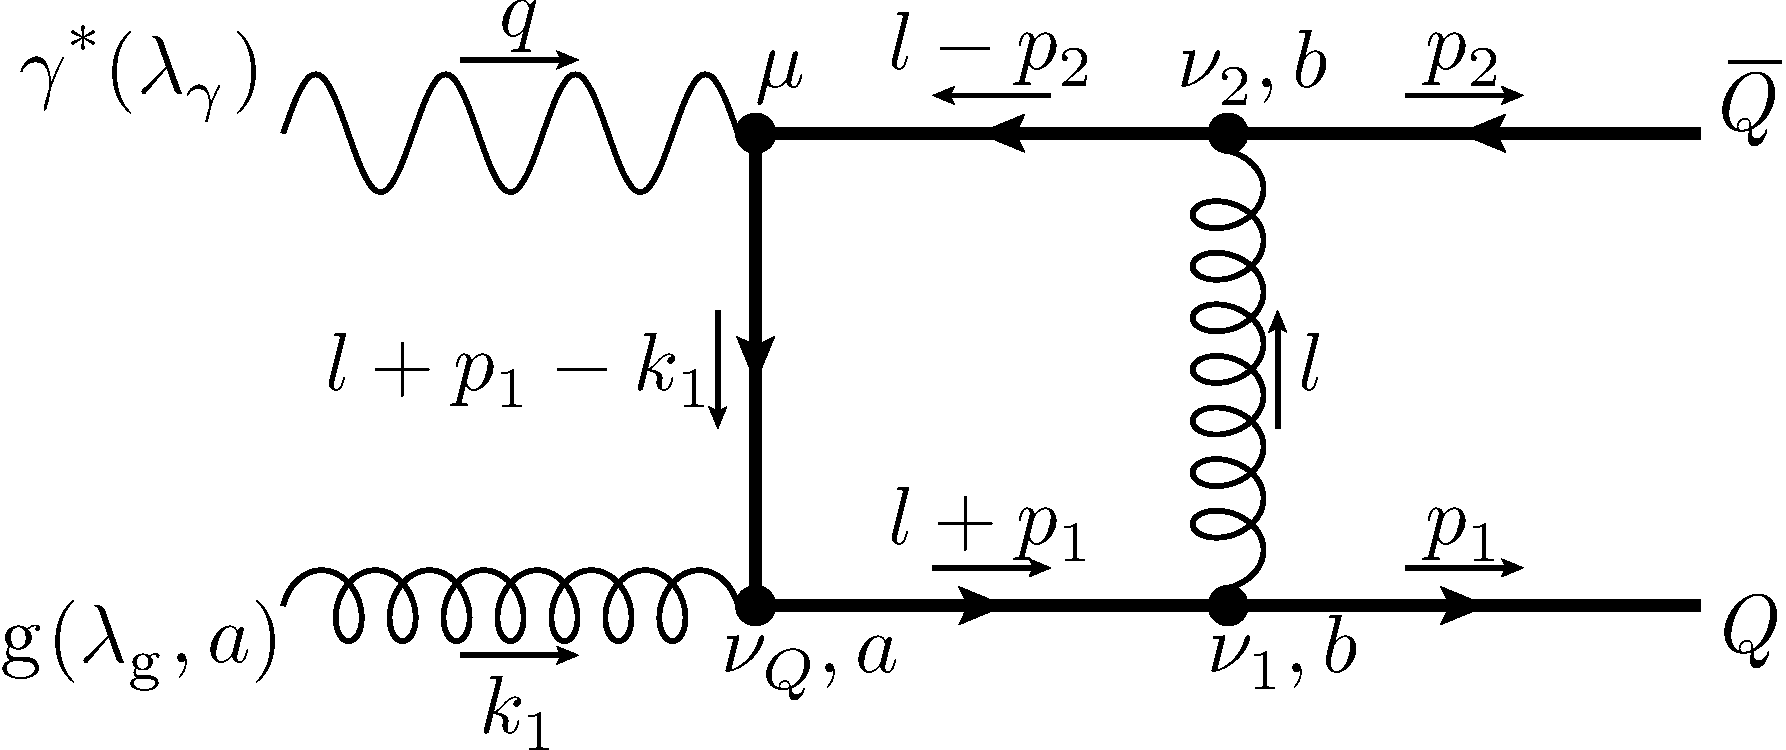
\includegraphics[width=\textwidth]{pyfeyn/nlo-v-box1}
		\caption{$i\Md^{(NLO,v)}_{1,\mu}$}
	\end{subfigure}\hspace{.15\textwidth}%
	\begin{subfigure}[t]{.4\textwidth}
		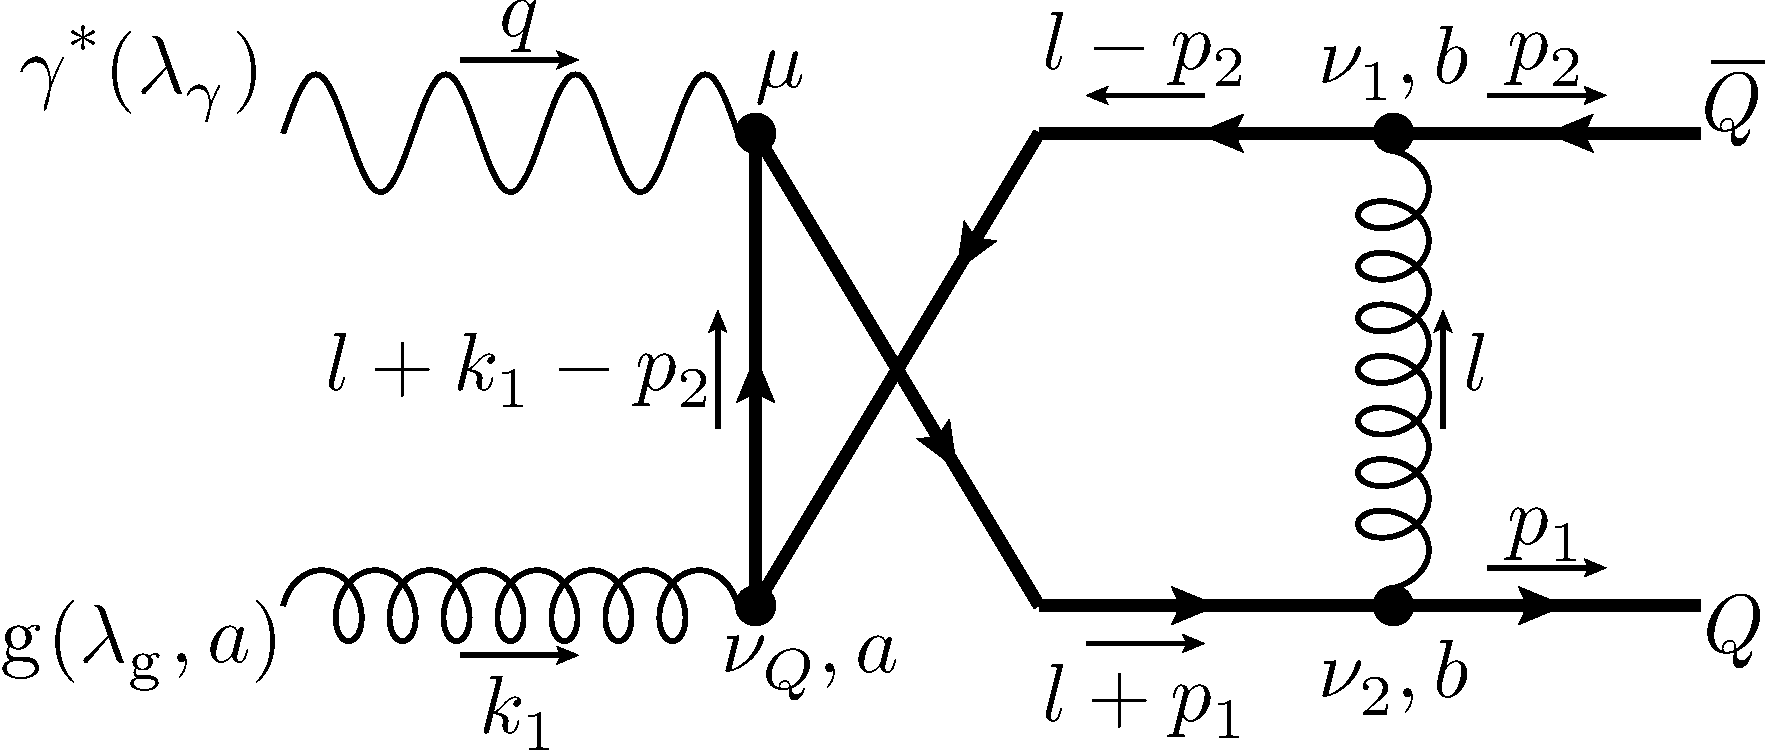
\includegraphics[width=\textwidth]{pyfeyn/nlo-v-box1cr}
		\caption{$i\Md^{(NLO,v)}_{2,\mu}$}
	\end{subfigure}\\
	\begin{subfigure}[t]{.6\textwidth}
		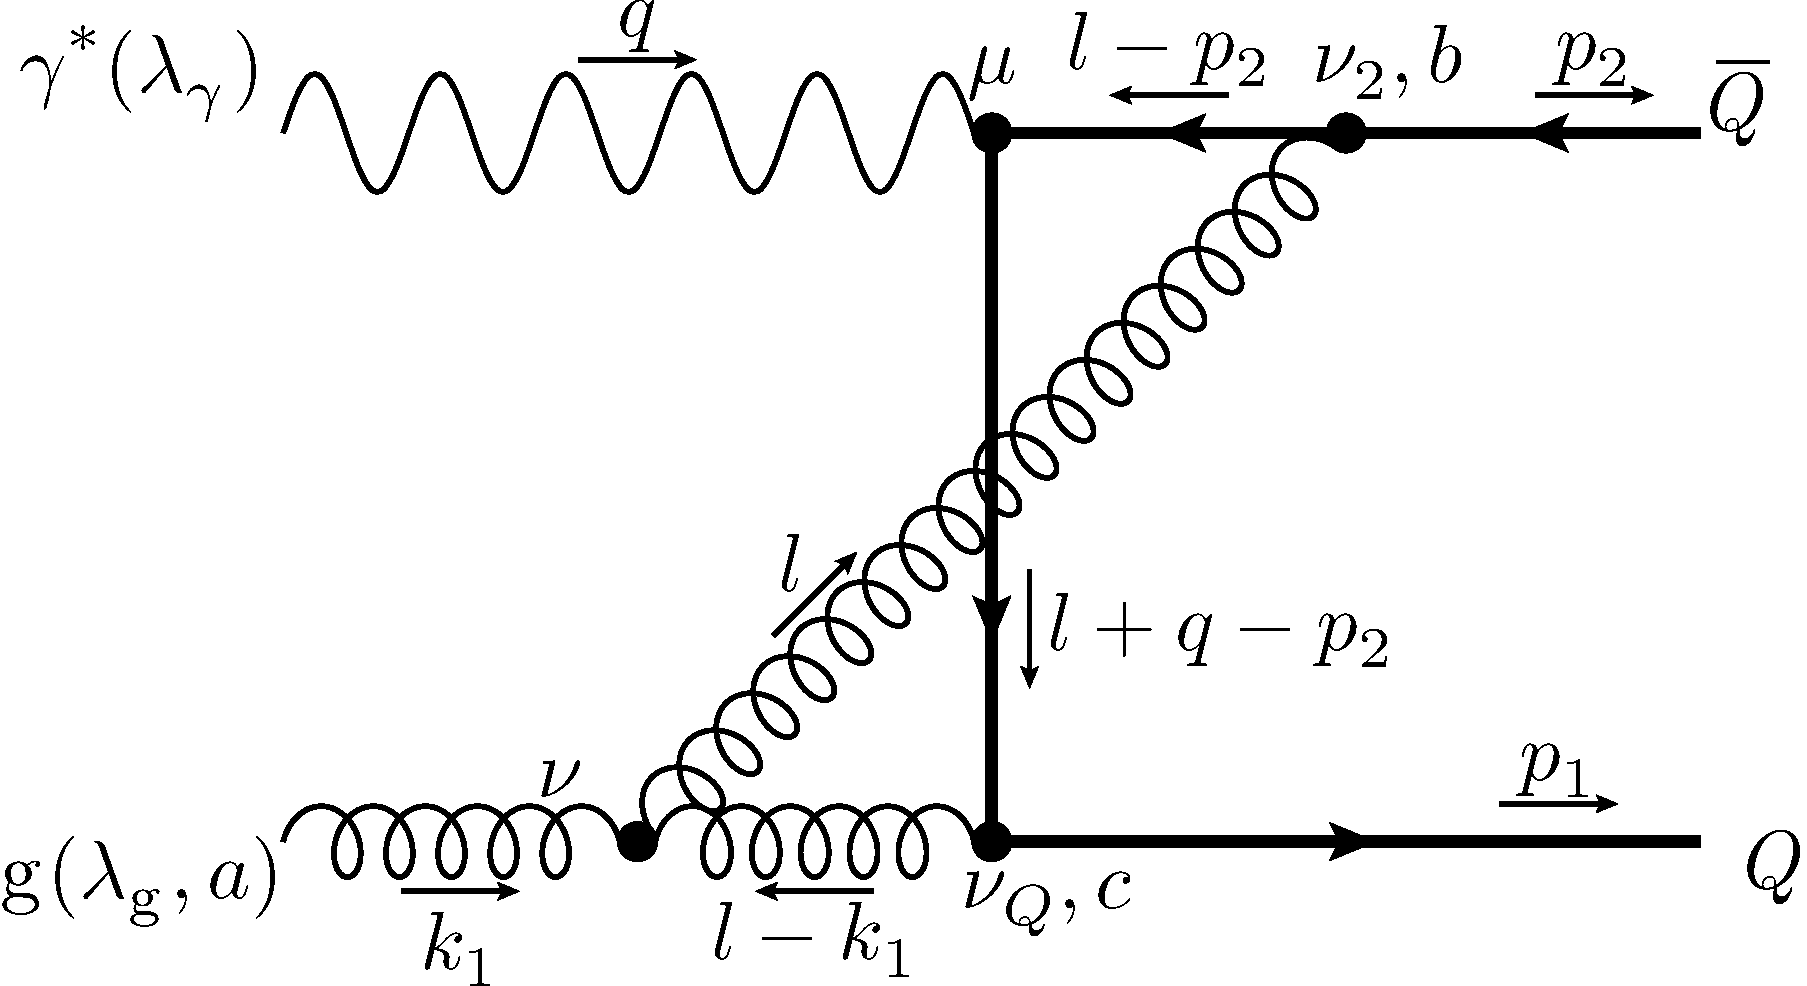
\includegraphics[width=\textwidth]{pyfeyn/nlo-v-box2}
		\caption{$i\Md^{(NLO,v)}_{3,\mu}$}
	\end{subfigure}
	\caption{NLO contributions by one loop}\label{fig:FeynNLOvab}
\end{figure}

\begin{align}
i\Md^{(NLO,v)}_{1,\mu} &=\mu_R^{4-n}\!\!\int\!\!\frac{d^nl}{(2\pi)^n}\,\bar u(p_1)(igT_b\gamma^{\nu_1})\frac{i(\slashed{l}+\slashed{p}_1+m)}{(l+p_1)^2-m^2}(igT_a\gamma^{\nu_Q})\frac{i(\slashed{l}+\slashed{p}_1-\slashed{k}_1+m)}{(l+p_1-k_1)^2-m^2}\cdot\nonumber\\
 &\hspace{40pt}(-i e e_H \gamma_\mu)\frac{i(\slashed{l}-\slashed{p}_2+m)}{(l-p_2)^2-m^2}(igT_b\gamma^{\nu_2})\frac{-ig_{\nu_1,\nu_2}}{l^2}v(p_2)\varepsilon^{(\lambda_{\Pg})}_{\nu_Q}(k_1)\\
i\Md^{(NLO,v)}_{2,\mu} &= \mu_R^{4-n}\!\!\int\!\!\frac{d^nl}{(2\pi)^n}\,\bar u(p_1)(igT_b\gamma^{\nu_1})\frac{i(\slashed{l}+\slashed{p}_1+m)}{(l+p_1)^2-m^2}(igT_a\gamma^{\nu_Q})\frac{i(\slashed{l}+\slashed{p}_1-\slashed{q}+m)}{(l+p_1-q)^2-m^2}\cdot\nonumber\\
 &\hspace{40pt}(-i e e_H \gamma_\mu)\frac{i(\slashed{l}-\slashed{p}_2+m)}{(l-p_2)^2-m^2}(igT_b\gamma^{\nu_2})\frac{-ig_{\nu_1,\nu_2}}{l^2}v(p_2)\varepsilon^{(\lambda_{\Pg})}_{\nu_Q}(k_1)\\
i\Md^{(NLO,v)}_{3,\mu} &=\mu_R^{4-n}\!\!\int\!\!\frac{d^nl}{(2\pi)^n}\,\bar u(p_1)(igT_c\gamma^{\nu_Q})\frac{i(\slashed{l}+\slashed{q}_1-\slashed{p}_2+m)}{(l+q-p_2)^2-m^2}(-i e e_H \gamma_\mu)\frac{i(\slashed{l}-\slashed{p}_2+m)}{(l-p_2)^2-m^2}\cdot\nonumber\\
 &\hspace{20pt}(igT_b\gamma^{\nu_2})\frac{(-i)^2}{l^2(l-k_1)^2}v(p_2)\varepsilon^{\nu,(\lambda_{\Pg})}(k_1)\cdot\nonumber\\
 &\hspace{20pt}\left(gf_{abc}\left(g_{\nu_2\nu_Q}(k_1-2l)_\nu+g_{\nu_Q\nu}(l-2k_1)_{\nu_2}+g_{\nu\nu_2}(k_1+l)_{\nu_Q}\right)\right)
\end{align}

\pagebreak

\begin{figure}[ht!]
	\begin{subfigure}[t]{.4\textwidth}
		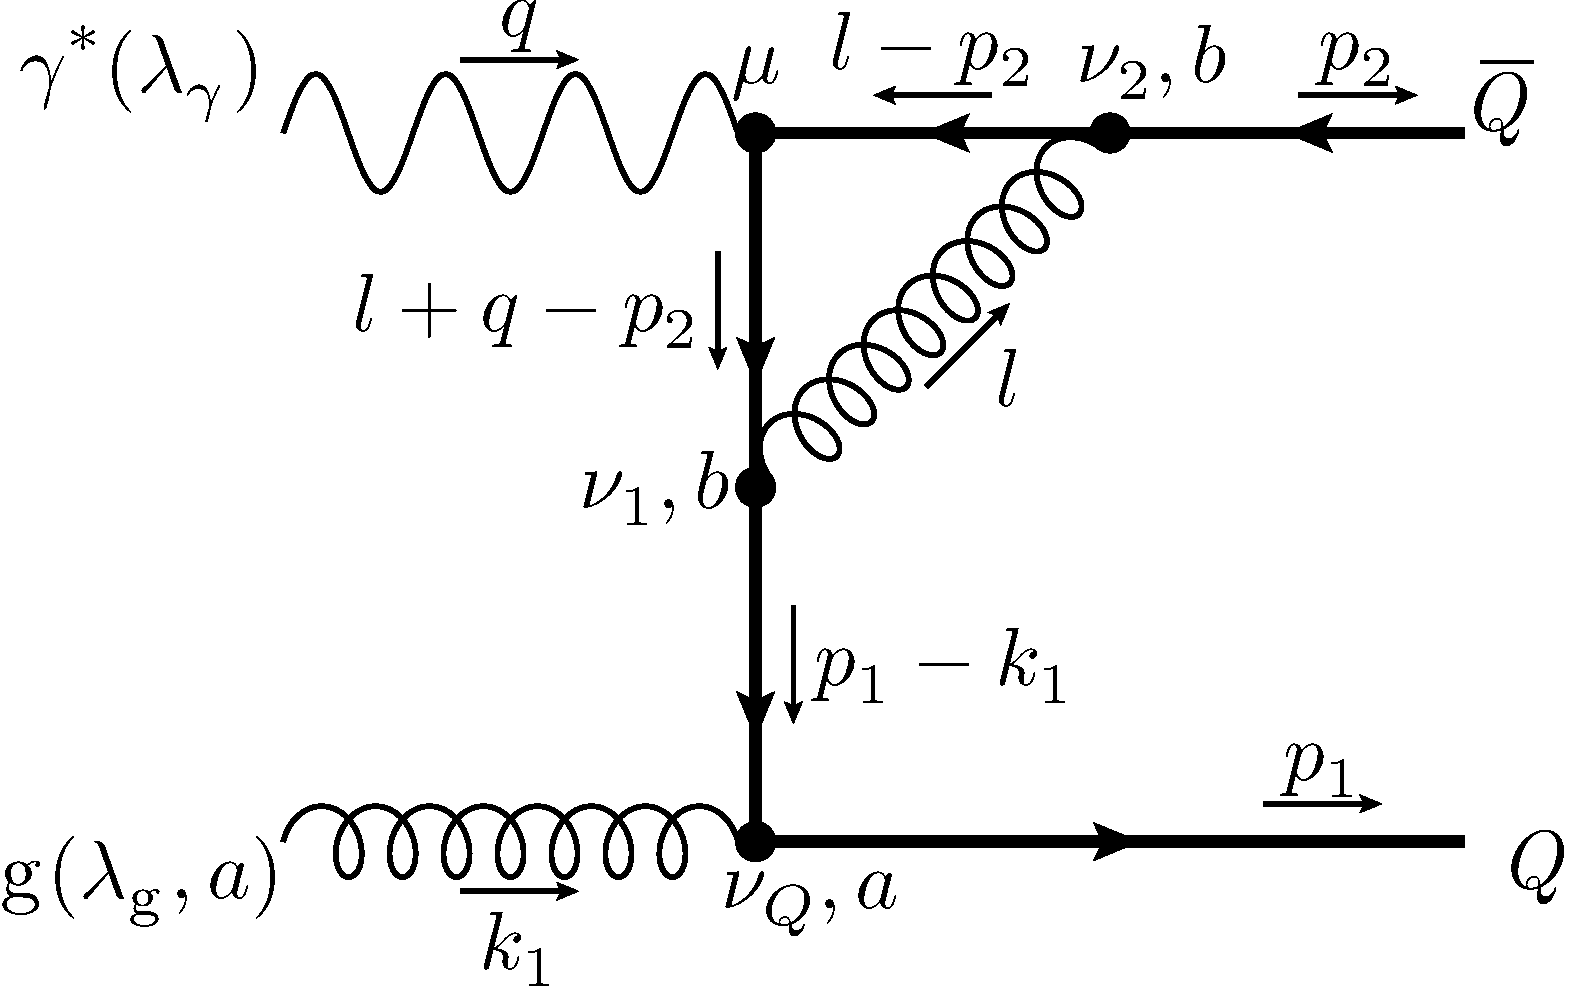
\includegraphics[width=\textwidth]{pyfeyn/nlo-v-e}
		\caption{$i\Md^{(NLO,v)}_{5,\mu}$}
	\end{subfigure}\hspace{.15\textwidth}%
	\begin{subfigure}[t]{.4\textwidth}
		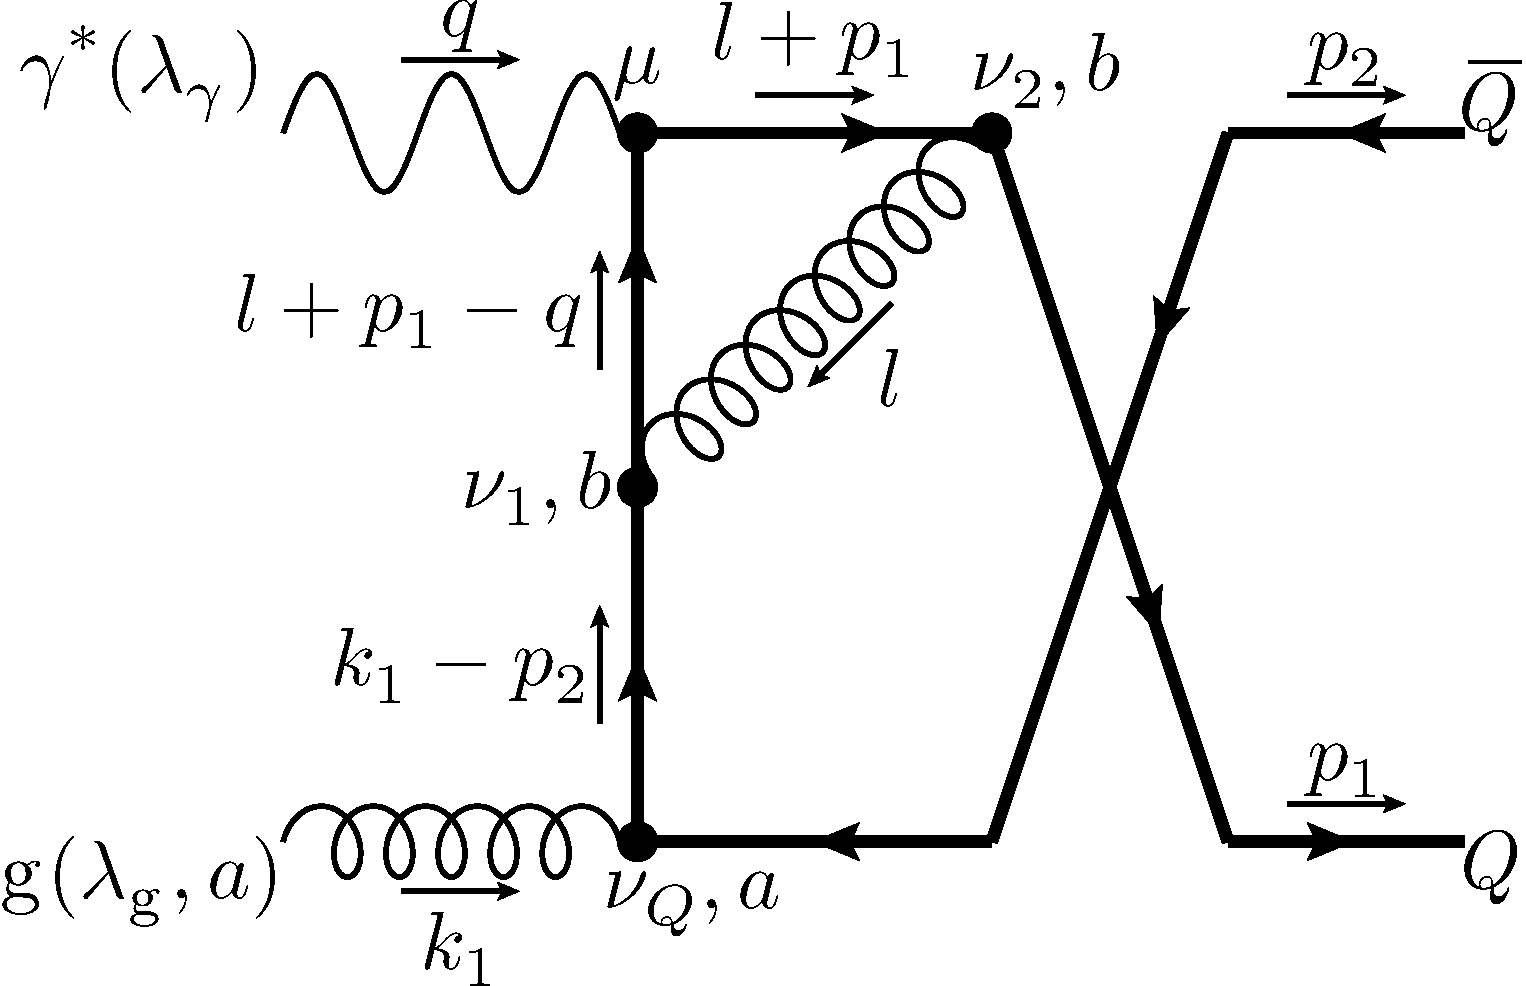
\includegraphics[width=\textwidth]{pyfeyn/nlo-v-ecr}
		\caption{$i\Md^{(NLO,v)}_{6,\mu}$}
	\end{subfigure}\\
	\begin{subfigure}[t]{.4\textwidth}
		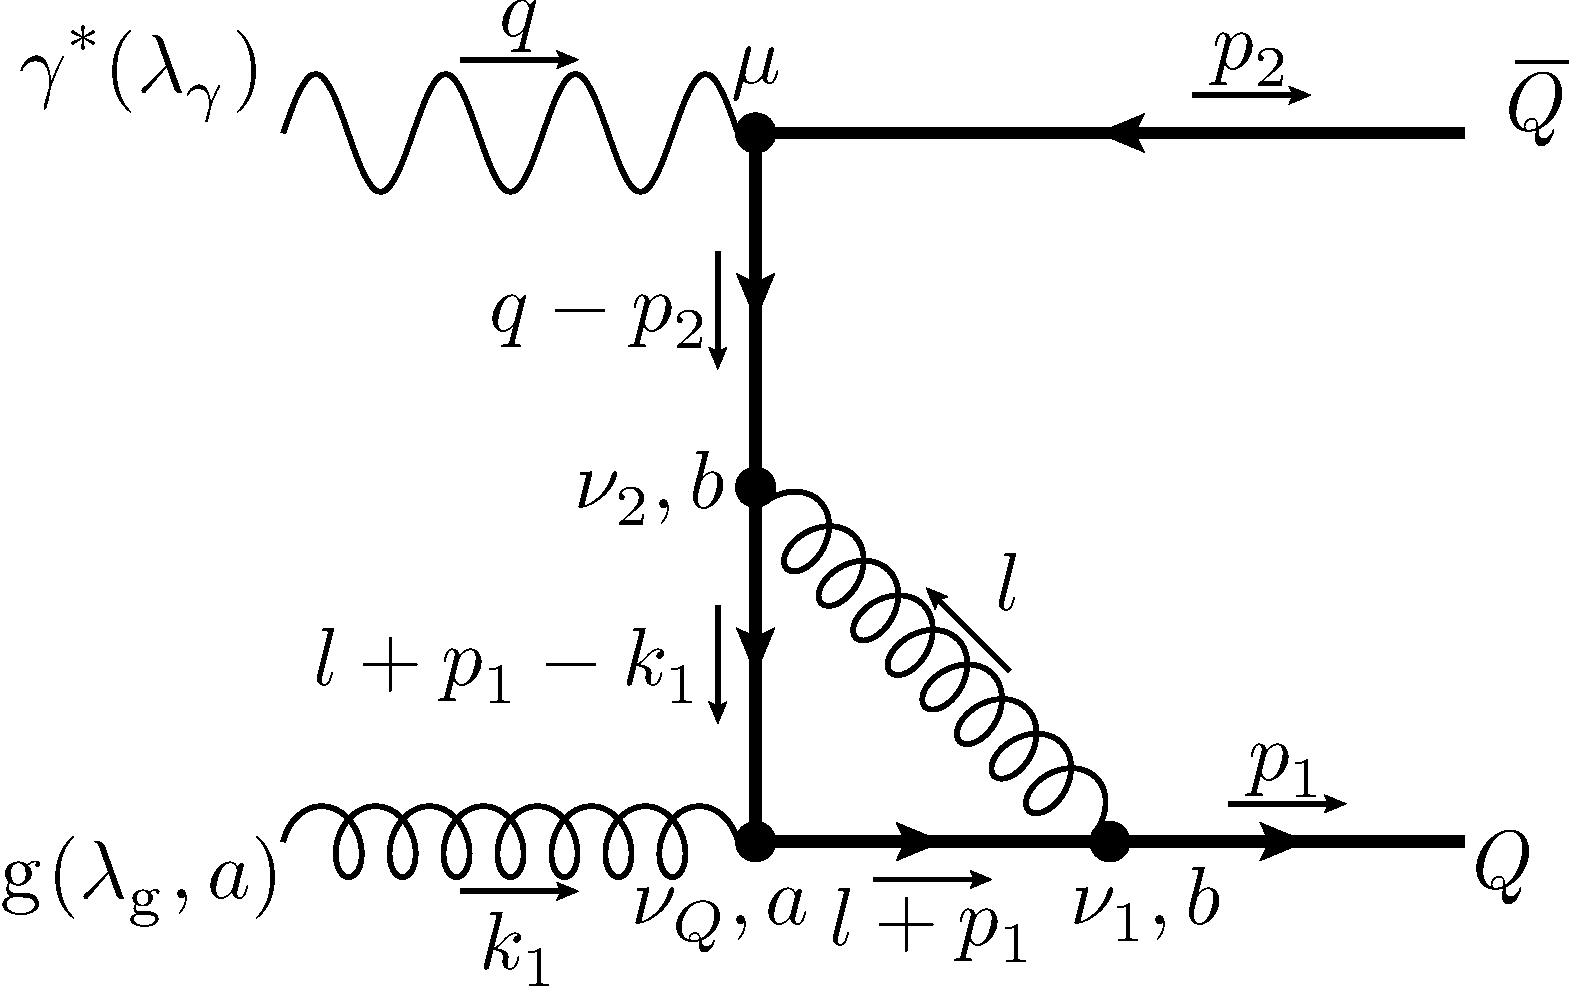
\includegraphics[width=\textwidth]{pyfeyn/nlo-v-g1}
		\caption{$i\Md^{(NLO,v)}_{7,\mu}$}
	\end{subfigure}\hspace{.15\textwidth}%
	\begin{subfigure}[t]{.4\textwidth}
		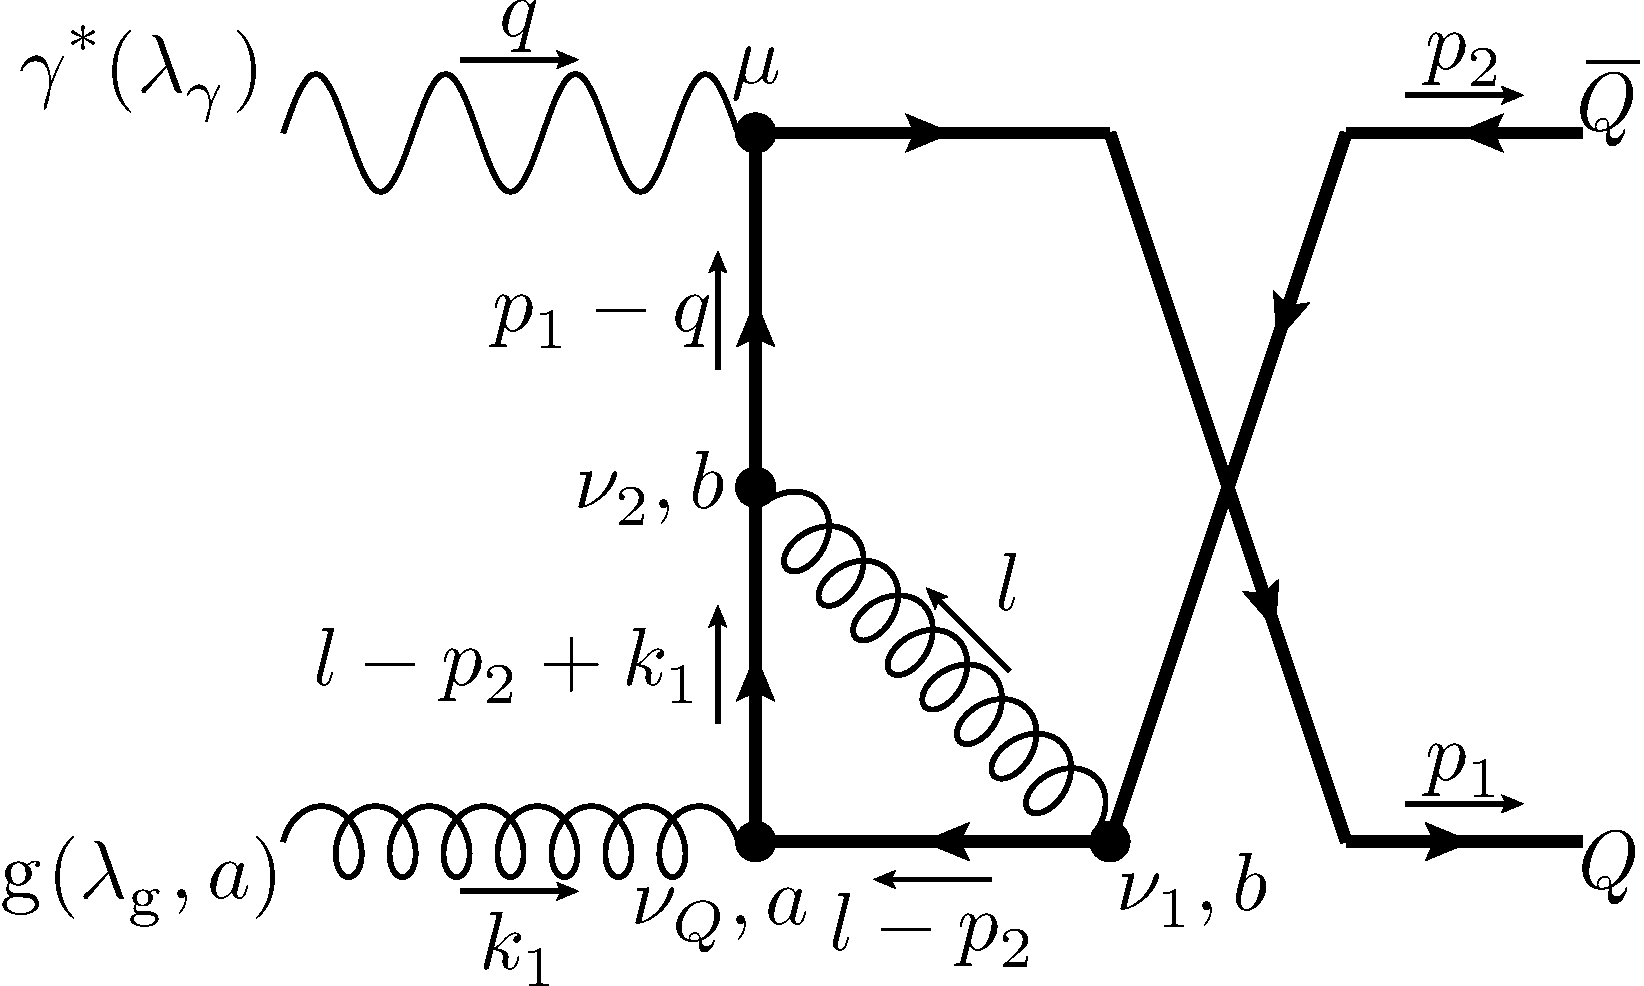
\includegraphics[width=\textwidth]{pyfeyn/nlo-v-g1cr}
		\caption{$i\Md^{(NLO,v)}_{8,\mu}$}
	\end{subfigure}
	\caption{NLO contributions by one loop (cont'ed)}\label{fig:FeynNLOvcd}
\end{figure}

\begin{align}
i\Md^{(NLO,v)}_{5,\mu} &=\mu_R^{4-n}\!\!\int\!\!\frac{d^nl}{(2\pi)^n}\,\bar u(p_1)(igT_a\gamma^{\nu_Q})\frac{i(\slashed{p}_1-\slashed{k}_1+m)}{u_1}(igT_b\gamma^{\nu_1})\frac{i(\slashed{l}+\slashed{q}-\slashed{p}_2+m)}{(l+q-p_2)^2-m^2}\cdot\nonumber\\
 &\hspace{40pt}(-i e e_H \gamma_\mu)\frac{i(\slashed{l}-\slashed{p}_2+m)}{(l-p_2)^2-m^2}(igT_b\gamma^{\nu_2})\frac{-ig_{\nu_1,\nu_2}}{l^2}v(p_2)\varepsilon^{(\lambda_{\Pg})}_{\nu_Q}(k_1)\\
i\Md^{(NLO,v)}_{6,\mu} &=\mu_R^{4-n}\!\!\int\!\!\frac{d^nl}{(2\pi)^n}\,\bar u(p_1)(igT_b\gamma^{\nu_2})\frac{i(\slashed{l}+\slashed{p}_1+m)}{(l+p_1)^2-m^2}(-i e e_H \gamma_\mu)\frac{i(\slashed{l}+\slashed{p}_1-\slashed{q}+m)}{(l+p_1-q)^2-m^2}\cdot\nonumber\\
 &\hspace{40pt}(igT_b\gamma^{\nu_1})\frac{i(\slashed{k}_1-\slashed{p}_2+m)}{t_1}(igT_a\gamma^{\nu_Q})\frac{-ig_{\nu_1,\nu_2}}{l^2}v(p_2)\varepsilon^{(\lambda_{\Pg})}_{\nu_Q}(k_1)\\
i\Md^{(NLO,v)}_{7,\mu} &=\mu_R^{4-n}\!\!\int\!\!\frac{d^nl}{(2\pi)^n}\,\bar u(p_1)(igT_b\gamma^{\nu_1})\frac{i(\slashed{l}+\slashed{p}_1+m)}{(l+p_1)^2-m^2}(igT_a\gamma^{\nu_Q})\frac{i(\slashed{l}+\slashed{p}_1-\slashed{k}_1+m)}{(l+p_1-k_1)^2-m^2}\cdot\nonumber\\
 &\hspace{40pt}(igT_b\gamma^{\nu_2})\frac{i(\slashed{q}-\slashed{p}_2+m)}{u_1}(-i e e_H \gamma_\mu)\frac{-ig_{\nu_1,\nu_2}}{l^2}v(p_2)\varepsilon^{(\lambda_{\Pg})}_{\nu_Q}(k_1)\\
i\Md^{(NLO,v)}_{8,\mu} &=\mu_R^{4-n}\!\!\int\!\!\frac{d^nl}{(2\pi)^n}\,\bar u(p_1)(-i e e_H \gamma_\mu)\frac{i(\slashed{p}_1-\slashed{q}+m)}{t_1}(igT_b\gamma^{\nu_2})\frac{i(\slashed{l}-\slashed{p}_2+\slashed{k}_1+m)}{(l-p_2+k_1)^2-m^2}\cdot\nonumber\\
 &\hspace{40pt}(igT_a\gamma^{\nu_Q})\frac{i(\slashed{l}-\slashed{p}_2+m)}{(l-p_2)^2-m^2}(igT_b\gamma^{\nu_1})\frac{-ig_{\nu_1,\nu_2}}{l^2}v(p_2)\varepsilon^{(\lambda_{\Pg})}_{\nu_Q}(k_1)
\end{align}

\pagebreak

\begin{figure}[ht!]
	\begin{subfigure}[t]{.4\textwidth}
		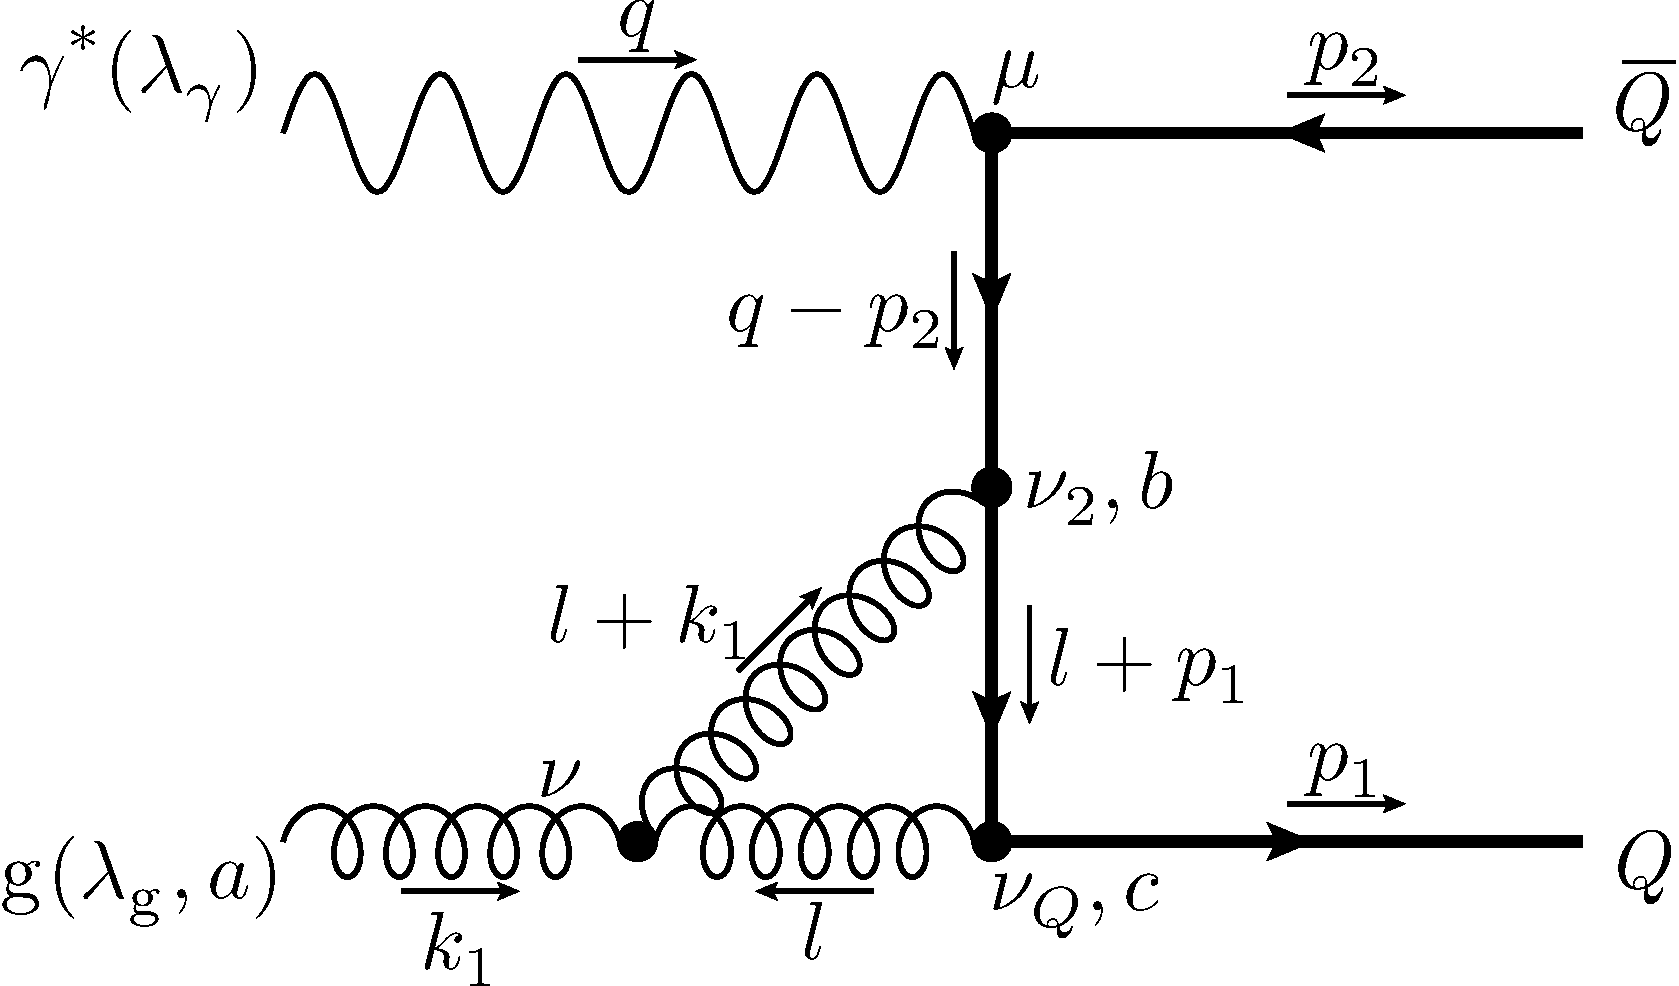
\includegraphics[width=\textwidth]{pyfeyn/nlo-v-g2}
		\caption{$i\Md^{(NLO,v)}_{9,\mu}$}
	\end{subfigure}\hspace{.15\textwidth}%
	\begin{subfigure}[t]{.4\textwidth}
		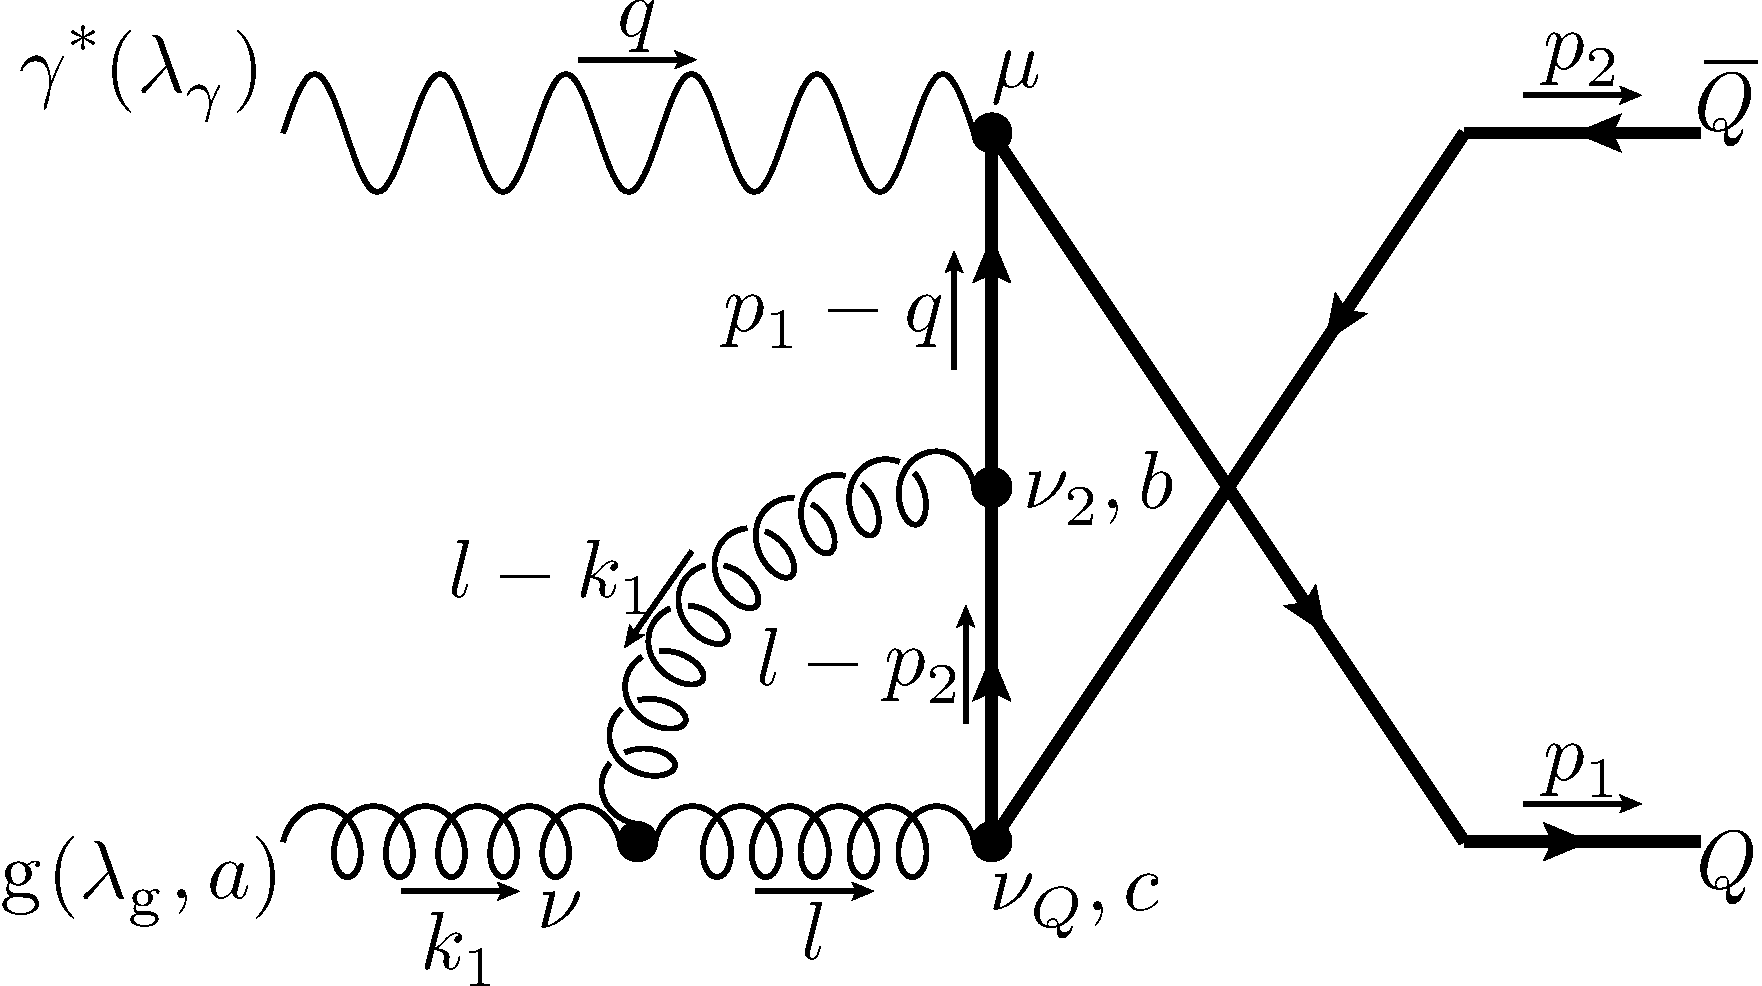
\includegraphics[width=\textwidth]{pyfeyn/nlo-v-g2cr}
		\caption{$i\Md^{(NLO,v)}_{10,\mu}$}
	\end{subfigure}\\
	\begin{subfigure}[t]{.4\textwidth}
		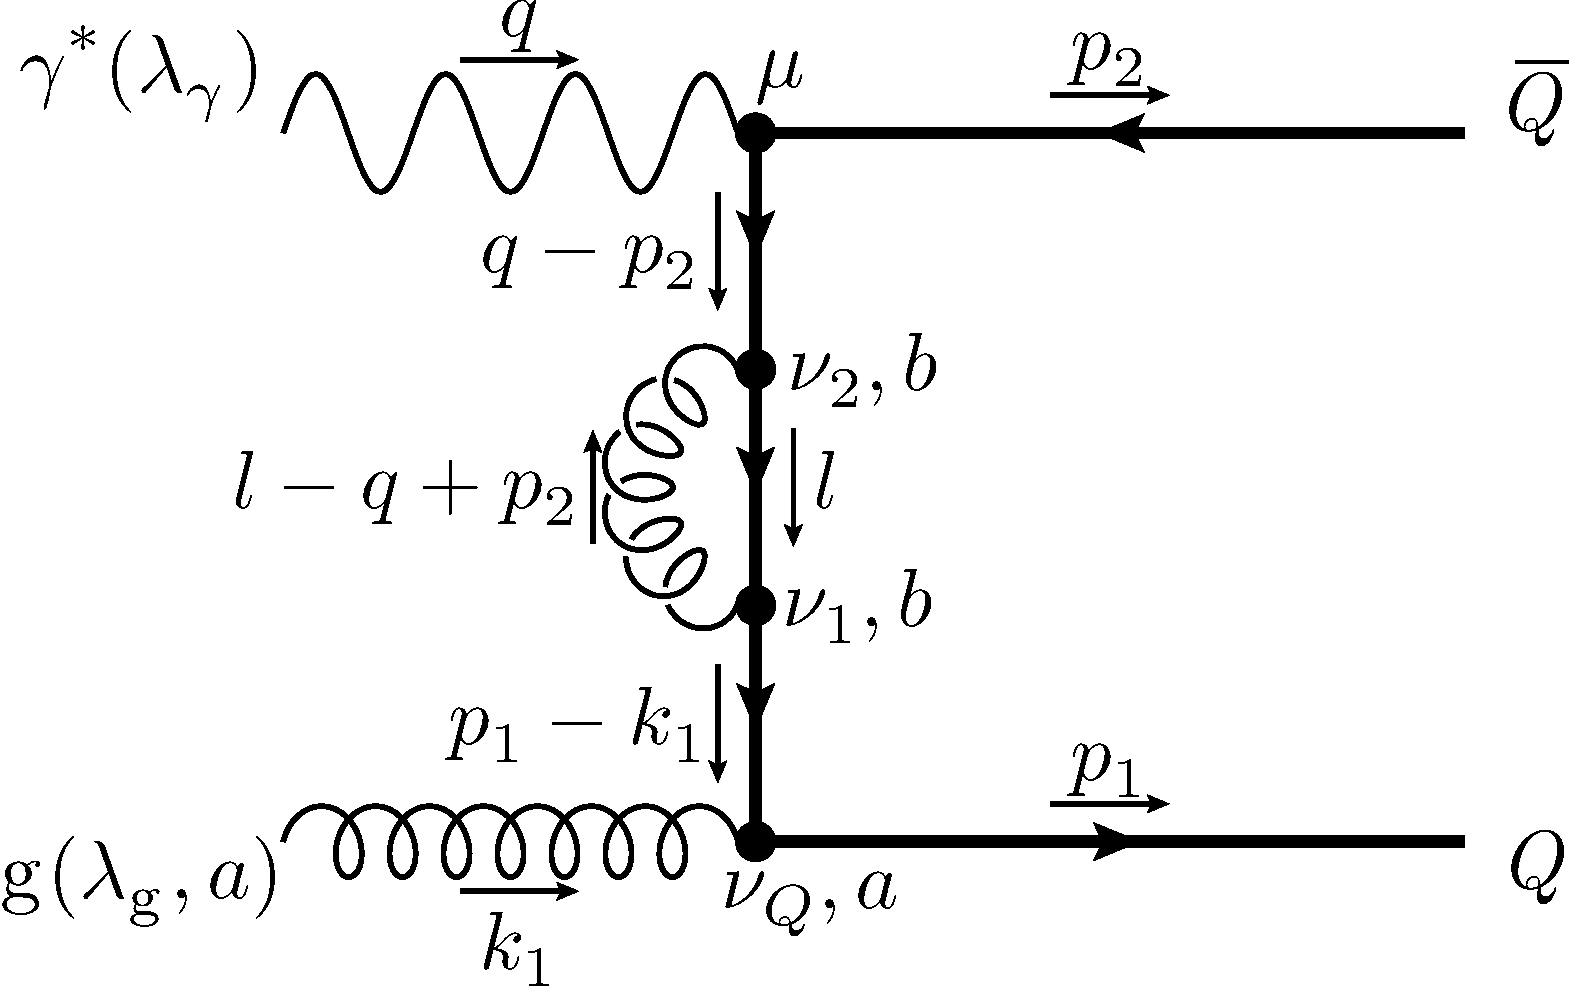
\includegraphics[width=\textwidth]{pyfeyn/nlo-v-m1}
		\caption{$i\Md^{(NLO,v)}_{11,\mu}$}
	\end{subfigure}\hspace{.15\textwidth}%
	\begin{subfigure}[t]{.4\textwidth}
		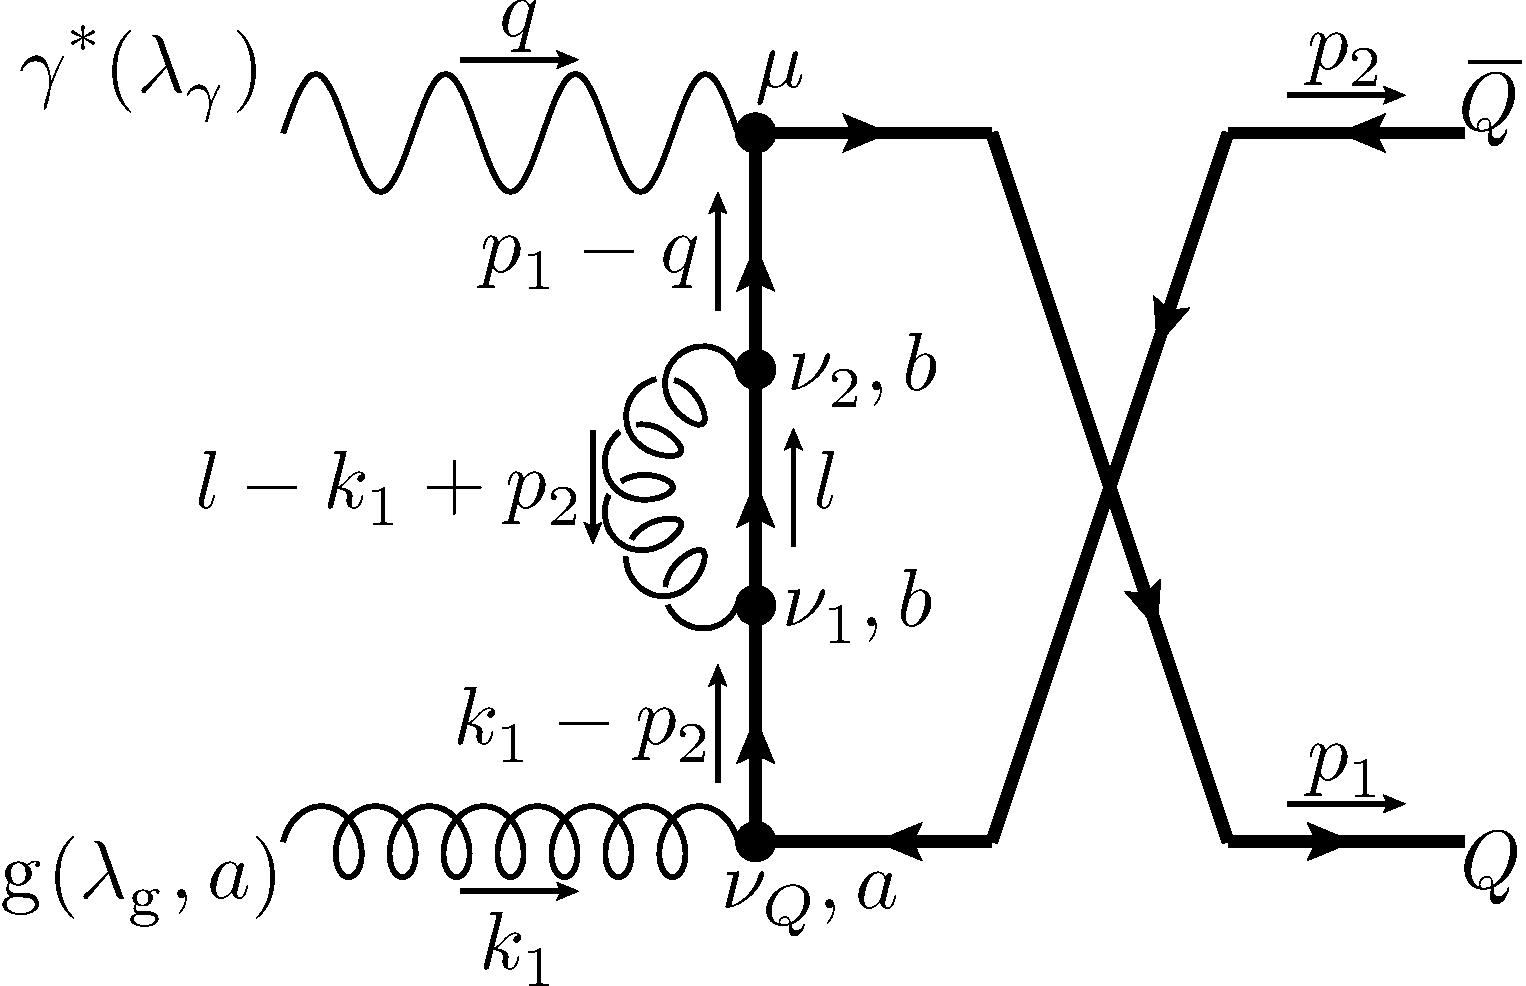
\includegraphics[width=\textwidth]{pyfeyn/nlo-v-m1cr}
		\caption{$i\Md^{(NLO,v)}_{12,\mu}$}
	\end{subfigure}
	\caption{NLO contributions by one loop (cont'ed)}\label{fig:FeynNLOve}
\end{figure}

\begin{align}
i\Md^{(NLO,v)}_{9,\mu} &=\mu_R^{4-n}\!\!\int\!\!\frac{d^nl}{(2\pi)^n}\,\bar u(p_1)(igT_c\gamma^{\nu_Q})\frac{i(\slashed{l}+\slashed{p}_1+m)}{(l+p_1)^2-m^2}(igT_b\gamma^{\nu_2})\frac{i(\slashed{q}-\slashed{p}_2+m)}{u_1}\cdot\nonumber\\
 &\hspace{20pt}(-i e e_H \gamma_\mu)\frac{(-i)^2}{l^2(l+k_1)^2}v(p_2)\varepsilon^{\nu,(\lambda_{\Pg})}(k_1)\cdot\nonumber\\
 &\hspace{20pt}\left(gf_{abc}\left(g_{\nu\nu_2}(2k_1+l)_{\nu_Q}+g_{\nu_2\nu_Q}(-2l-k_1)_{\nu}+g_{\nu_Q\nu}(l-k_1)_{\nu_2}\right)\right)\\
i\Md^{(NLO,v)}_{10,\mu} &=\mu_R^{4-n}\!\!\int\!\!\frac{d^nl}{(2\pi)^n}\,\bar u(p_1)(-i e e_H \gamma_\mu)\frac{i(\slashed{p}_1-\slashed{q}+m)}{t_1}(igT_b\gamma^{\nu_2})\frac{i(\slashed{l}-\slashed{p}_2+m)}{(l-p_2)^2-m^2}\cdot\nonumber\\
 &\hspace{20pt}(igT_c\gamma^{\nu_Q})\frac{(-i)^2}{l^2(l-k_1)^2}v(p_2)\varepsilon^{\nu,(\lambda_{\Pg})}(k_1)\cdot\nonumber\\
 &\hspace{20pt}\left(gf_{abc}\left(g_{\nu\nu_2}(2k_1-l)_{\nu_Q}+g_{\nu_2\nu_Q}(2l-k_1)_{\nu}+g_{\nu_Q\nu}(-l-k_1)_{\nu_2}\right)\right)\\
i\Md^{(NLO,v)}_{11,\mu} &=\mu_R^{4-n}\!\!\int\!\!\frac{d^nl}{(2\pi)^n}\,\bar u(p_1)(igT_a\gamma^{\nu_Q})\frac{i(\slashed{p}_1-\slashed{k}_1+m)}{u_1}(igT_b\gamma^{\nu_1})\frac{i(\slashed{l}+m)}{l^2-m^2}\cdot\nonumber\\
 &\hspace{40pt}(igT_b\gamma^{\nu_2})\frac{i(\slashed{q}-\slashed{p}_2+m)}{u_1}(-i e e_H \gamma_\mu)\frac{-ig_{\nu_1,\nu_2}}{(l-q+p_2)^2}v(p_2)\varepsilon^{(\lambda_{\Pg})}_{\nu_Q}(k_1)\\
i\Md^{(NLO,v)}_{12,\mu} &=\mu^{4-n}\!\!\int\!\!\frac{d^nl}{(2\pi)^n}\,\bar u(p_1)(-i e e_H \gamma_\mu)\frac{i(\slashed{p}_1-\slashed{q}+m)}{t_1}(igT_b\gamma^{\nu_2})\frac{i(\slashed{l}+m)}{l^2-m^2}\cdot\nonumber\\
 &\hspace{40pt}(igT_b\gamma^{\nu_1})\frac{i(\slashed{k}_1-\slashed{p}_2+m)}{t_1}(igT_a\gamma^{\nu_Q})\frac{-ig_{\nu_1,\nu_2}}{(l-k_1+p_2)^2}v(p_2)\varepsilon^{(\lambda_{\Pg})}_{\nu_Q}(k_1)
\end{align}

Color space:
\begin{align}
&\left(\Md^{(NLO,v)}_{1,\mu}+\Md^{(NLO,v)}_{2,\mu} + \Md^{(NLO,v)}_{7,\mu}+\Md^{(NLO,v)}_{8,\mu}\right)\nonumber\\
&\hspace{20pt}\cdot\left(\Md^{(LO)}_{1,\mu'}+\Md^{(LO)}_{2,\mu'}\right)^*\sim -i\tr(T_aT_bT_aT_b) = -iN_C C_F \left(C_F - \frac{C_A}{2}\right)\\
&\left(\Md^{(NLO,v)}_{3,\mu}+ \Md^{(NLO,v)}_{9,\mu}+\Md^{(NLO,v)}_{10,\mu}\right)\nonumber\\
&\hspace{20pt}\cdot\left(\Md^{(LO)}_{1,\mu'}+\Md^{(LO)}_{2,\mu'}\right)^*\sim f_{abc}\tr(T_cT_bT_a) = -\frac i 2 N_C C_F C_A\\
&\left(\Md^{(NLO,v)}_{5,\mu}+\Md^{(NLO,v)}_{6,\mu}+\Md^{(NLO,v)}_{11,\mu}+\Md^{(NLO,v)}_{12,\mu}\right)\nonumber\\
&\hspace{20pt}\cdot\left(\Md^{(LO)}_{1,\mu'}+\Md^{(LO)}_{2,\mu'}\right)^*\sim -i\tr(T_aT_aT_bT_b) = -iN_C C_F^2
\end{align}
